  
\documentclass{article}
\usepackage[spanish]{babel}
\usepackage[numbers,sort&compress]{natbib}
\usepackage{graphicx}

\title{Pr\'{a}ctica 2: auto\'{a}mata celular}
\author{Isaac Estrada Garc\'{i}a }

\begin{document}

\maketitle



\section{Hip\'{o}tesis}
El colapso poblacional ser\'{a} evidente entre la primera y segunda iteraci\'{o}n. 
\section{Objetivos}
Dise\~{n}ar y ejecutar \citep{elis} un experimento aut\'{o}mata celular, particularmente el juego de la vida para determinar el mayor colapso poblacional entre iteraciones subsecuentes en una malla de 50 por 50 celdas hasta que mueran todas, variando la probabilidad inicial entre 0.1 y 0.9 en pasos de 0.1. Cada celda est\'{a} representada por una variable booleana es decir ceros y unos donde, viva representa un uno y muerta un cero, la regla del juego es: la celda vive si solo tres vecinos est�n vivos.

\section{Simulaci\'{o}n y Resultados}

La simulaci\'{o}n del experimento arroja im\'{a}genes donde a menor probabilidad poblacional inicial   menor es el colapso poblacional hasta llegar a probabilidad = 0.5 donde llega a su punto m\'{a}ximo como en la \ref{fig} y de ah� decrece. En el repositorio de simulaci�n se encuentra los archivos .gif de la simulaci\'{o}n

En la figura \ref{fig} se muestran los resultados obtenidos por la simulaci\'{o}n, donde se puede observar una tendencia decreciente de regresos al origen conforme aumentan las dimenciones.


\begin{figure}
  \centering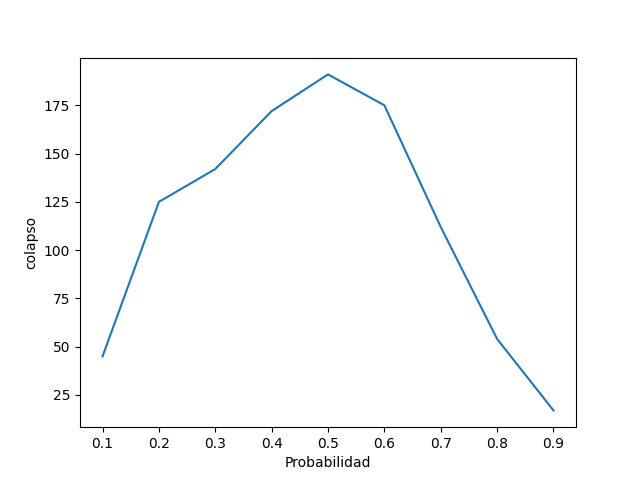
\includegraphics[width=0.9\textwidth]{colapso.png}
  \caption{Colapso poblacional de juego de la vida variando su probabilidad inicial.}
  \label{fig}
\end{figure} 



\section{Conclusi\'{o}n}

El mayor colapso poblacional sucede en la probabilidad igual a 0.5 inicial de la poblaci\'{o}n pues es donde hay mejor distribuci\'{o}n de c\'{e}lulas vivas y esto lo beneficia.

\bibliography{p2}
\bibliographystyle{plainnat}
 
\end{document}
